% Options for packages loaded elsewhere
\PassOptionsToPackage{unicode}{hyperref}
\PassOptionsToPackage{hyphens}{url}
\PassOptionsToPackage{dvipsnames,svgnames,x11names}{xcolor}
%
\documentclass[
  letterpaper,
  DIV=11,
  numbers=noendperiod]{scrreprt}

\usepackage{amsmath,amssymb}
\usepackage{iftex}
\ifPDFTeX
  \usepackage[T1]{fontenc}
  \usepackage[utf8]{inputenc}
  \usepackage{textcomp} % provide euro and other symbols
\else % if luatex or xetex
  \usepackage{unicode-math}
  \defaultfontfeatures{Scale=MatchLowercase}
  \defaultfontfeatures[\rmfamily]{Ligatures=TeX,Scale=1}
\fi
\usepackage{lmodern}
\ifPDFTeX\else  
    % xetex/luatex font selection
\fi
% Use upquote if available, for straight quotes in verbatim environments
\IfFileExists{upquote.sty}{\usepackage{upquote}}{}
\IfFileExists{microtype.sty}{% use microtype if available
  \usepackage[]{microtype}
  \UseMicrotypeSet[protrusion]{basicmath} % disable protrusion for tt fonts
}{}
\makeatletter
\@ifundefined{KOMAClassName}{% if non-KOMA class
  \IfFileExists{parskip.sty}{%
    \usepackage{parskip}
  }{% else
    \setlength{\parindent}{0pt}
    \setlength{\parskip}{6pt plus 2pt minus 1pt}}
}{% if KOMA class
  \KOMAoptions{parskip=half}}
\makeatother
\usepackage{xcolor}
\setlength{\emergencystretch}{3em} % prevent overfull lines
\setcounter{secnumdepth}{5}
% Make \paragraph and \subparagraph free-standing
\ifx\paragraph\undefined\else
  \let\oldparagraph\paragraph
  \renewcommand{\paragraph}[1]{\oldparagraph{#1}\mbox{}}
\fi
\ifx\subparagraph\undefined\else
  \let\oldsubparagraph\subparagraph
  \renewcommand{\subparagraph}[1]{\oldsubparagraph{#1}\mbox{}}
\fi

\usepackage{color}
\usepackage{fancyvrb}
\newcommand{\VerbBar}{|}
\newcommand{\VERB}{\Verb[commandchars=\\\{\}]}
\DefineVerbatimEnvironment{Highlighting}{Verbatim}{commandchars=\\\{\}}
% Add ',fontsize=\small' for more characters per line
\usepackage{framed}
\definecolor{shadecolor}{RGB}{241,243,245}
\newenvironment{Shaded}{\begin{snugshade}}{\end{snugshade}}
\newcommand{\AlertTok}[1]{\textcolor[rgb]{0.68,0.00,0.00}{#1}}
\newcommand{\AnnotationTok}[1]{\textcolor[rgb]{0.37,0.37,0.37}{#1}}
\newcommand{\AttributeTok}[1]{\textcolor[rgb]{0.40,0.45,0.13}{#1}}
\newcommand{\BaseNTok}[1]{\textcolor[rgb]{0.68,0.00,0.00}{#1}}
\newcommand{\BuiltInTok}[1]{\textcolor[rgb]{0.00,0.23,0.31}{#1}}
\newcommand{\CharTok}[1]{\textcolor[rgb]{0.13,0.47,0.30}{#1}}
\newcommand{\CommentTok}[1]{\textcolor[rgb]{0.37,0.37,0.37}{#1}}
\newcommand{\CommentVarTok}[1]{\textcolor[rgb]{0.37,0.37,0.37}{\textit{#1}}}
\newcommand{\ConstantTok}[1]{\textcolor[rgb]{0.56,0.35,0.01}{#1}}
\newcommand{\ControlFlowTok}[1]{\textcolor[rgb]{0.00,0.23,0.31}{#1}}
\newcommand{\DataTypeTok}[1]{\textcolor[rgb]{0.68,0.00,0.00}{#1}}
\newcommand{\DecValTok}[1]{\textcolor[rgb]{0.68,0.00,0.00}{#1}}
\newcommand{\DocumentationTok}[1]{\textcolor[rgb]{0.37,0.37,0.37}{\textit{#1}}}
\newcommand{\ErrorTok}[1]{\textcolor[rgb]{0.68,0.00,0.00}{#1}}
\newcommand{\ExtensionTok}[1]{\textcolor[rgb]{0.00,0.23,0.31}{#1}}
\newcommand{\FloatTok}[1]{\textcolor[rgb]{0.68,0.00,0.00}{#1}}
\newcommand{\FunctionTok}[1]{\textcolor[rgb]{0.28,0.35,0.67}{#1}}
\newcommand{\ImportTok}[1]{\textcolor[rgb]{0.00,0.46,0.62}{#1}}
\newcommand{\InformationTok}[1]{\textcolor[rgb]{0.37,0.37,0.37}{#1}}
\newcommand{\KeywordTok}[1]{\textcolor[rgb]{0.00,0.23,0.31}{#1}}
\newcommand{\NormalTok}[1]{\textcolor[rgb]{0.00,0.23,0.31}{#1}}
\newcommand{\OperatorTok}[1]{\textcolor[rgb]{0.37,0.37,0.37}{#1}}
\newcommand{\OtherTok}[1]{\textcolor[rgb]{0.00,0.23,0.31}{#1}}
\newcommand{\PreprocessorTok}[1]{\textcolor[rgb]{0.68,0.00,0.00}{#1}}
\newcommand{\RegionMarkerTok}[1]{\textcolor[rgb]{0.00,0.23,0.31}{#1}}
\newcommand{\SpecialCharTok}[1]{\textcolor[rgb]{0.37,0.37,0.37}{#1}}
\newcommand{\SpecialStringTok}[1]{\textcolor[rgb]{0.13,0.47,0.30}{#1}}
\newcommand{\StringTok}[1]{\textcolor[rgb]{0.13,0.47,0.30}{#1}}
\newcommand{\VariableTok}[1]{\textcolor[rgb]{0.07,0.07,0.07}{#1}}
\newcommand{\VerbatimStringTok}[1]{\textcolor[rgb]{0.13,0.47,0.30}{#1}}
\newcommand{\WarningTok}[1]{\textcolor[rgb]{0.37,0.37,0.37}{\textit{#1}}}

\providecommand{\tightlist}{%
  \setlength{\itemsep}{0pt}\setlength{\parskip}{0pt}}\usepackage{longtable,booktabs,array}
\usepackage{calc} % for calculating minipage widths
% Correct order of tables after \paragraph or \subparagraph
\usepackage{etoolbox}
\makeatletter
\patchcmd\longtable{\par}{\if@noskipsec\mbox{}\fi\par}{}{}
\makeatother
% Allow footnotes in longtable head/foot
\IfFileExists{footnotehyper.sty}{\usepackage{footnotehyper}}{\usepackage{footnote}}
\makesavenoteenv{longtable}
\usepackage{graphicx}
\makeatletter
\def\maxwidth{\ifdim\Gin@nat@width>\linewidth\linewidth\else\Gin@nat@width\fi}
\def\maxheight{\ifdim\Gin@nat@height>\textheight\textheight\else\Gin@nat@height\fi}
\makeatother
% Scale images if necessary, so that they will not overflow the page
% margins by default, and it is still possible to overwrite the defaults
% using explicit options in \includegraphics[width, height, ...]{}
\setkeys{Gin}{width=\maxwidth,height=\maxheight,keepaspectratio}
% Set default figure placement to htbp
\makeatletter
\def\fps@figure{htbp}
\makeatother

\KOMAoption{captions}{tableheading}
\makeatletter
\@ifpackageloaded{bookmark}{}{\usepackage{bookmark}}
\makeatother
\makeatletter
\@ifpackageloaded{caption}{}{\usepackage{caption}}
\AtBeginDocument{%
\ifdefined\contentsname
  \renewcommand*\contentsname{Table of contents}
\else
  \newcommand\contentsname{Table of contents}
\fi
\ifdefined\listfigurename
  \renewcommand*\listfigurename{List of Figures}
\else
  \newcommand\listfigurename{List of Figures}
\fi
\ifdefined\listtablename
  \renewcommand*\listtablename{List of Tables}
\else
  \newcommand\listtablename{List of Tables}
\fi
\ifdefined\figurename
  \renewcommand*\figurename{Figure}
\else
  \newcommand\figurename{Figure}
\fi
\ifdefined\tablename
  \renewcommand*\tablename{Table}
\else
  \newcommand\tablename{Table}
\fi
}
\@ifpackageloaded{float}{}{\usepackage{float}}
\floatstyle{ruled}
\@ifundefined{c@chapter}{\newfloat{codelisting}{h}{lop}}{\newfloat{codelisting}{h}{lop}[chapter]}
\floatname{codelisting}{Listing}
\newcommand*\listoflistings{\listof{codelisting}{List of Listings}}
\makeatother
\makeatletter
\makeatother
\makeatletter
\@ifpackageloaded{caption}{}{\usepackage{caption}}
\@ifpackageloaded{subcaption}{}{\usepackage{subcaption}}
\makeatother
\ifLuaTeX
  \usepackage{selnolig}  % disable illegal ligatures
\fi
\usepackage{bookmark}

\IfFileExists{xurl.sty}{\usepackage{xurl}}{} % add URL line breaks if available
\urlstyle{same} % disable monospaced font for URLs
\hypersetup{
  pdftitle={Notebook},
  pdfauthor={Norah Jones},
  colorlinks=true,
  linkcolor={blue},
  filecolor={Maroon},
  citecolor={Blue},
  urlcolor={Blue},
  pdfcreator={LaTeX via pandoc}}

\title{Notebook}
\author{Norah Jones}
\date{2025-01-23}

\begin{document}
\maketitle

\renewcommand*\contentsname{Table of contents}
{
\hypersetup{linkcolor=}
\setcounter{tocdepth}{2}
\tableofcontents
}
\bookmarksetup{startatroot}

\chapter*{Preface}\label{preface}
\addcontentsline{toc}{chapter}{Preface}

\markboth{Preface}{Preface}

This is a Quarto book.

To learn more about Quarto books visit
\url{https://quarto.org/docs/books}.

\bookmarksetup{startatroot}

\chapter{Apr.~12, 2021 (Mixed models)}\label{apr.-12-2021-mixed-models}

Source: 2021-04-12-models.rmarkdown

We fit two mixed models on the sleep dataset using brms.

One with random intercepts:

\begin{Shaded}
\begin{Highlighting}[]
\FunctionTok{library}\NormalTok{(tidyverse)}
\end{Highlighting}
\end{Shaded}

\begin{verbatim}
-- Attaching core tidyverse packages ------------------------ tidyverse 2.0.0 --
v dplyr     1.1.4     v readr     2.1.5
v forcats   1.0.0     v stringr   1.5.1
v ggplot2   3.5.1     v tibble    3.2.1
v lubridate 1.9.4     v tidyr     1.3.1
v purrr     1.0.2     
-- Conflicts ------------------------------------------ tidyverse_conflicts() --
x dplyr::filter() masks stats::filter()
x dplyr::lag()    masks stats::lag()
i Use the conflicted package (<http://conflicted.r-lib.org/>) to force all conflicts to become errors
\end{verbatim}

\begin{Shaded}
\begin{Highlighting}[]
\FunctionTok{library}\NormalTok{(brms)}
\end{Highlighting}
\end{Shaded}

\begin{verbatim}
Loading required package: Rcpp
Loading 'brms' package (version 2.22.0). Useful instructions
can be found by typing help('brms'). A more detailed introduction
to the package is available through vignette('brms_overview').

Attaching package: 'brms'

The following object is masked from 'package:stats':

    ar
\end{verbatim}

\begin{Shaded}
\begin{Highlighting}[]
\NormalTok{model\_1 }\OtherTok{\textless{}{-}}\NormalTok{ targets}\SpecialCharTok{::}\FunctionTok{tar\_read}\NormalTok{(model\_1)}
\NormalTok{model\_2 }\OtherTok{\textless{}{-}}\NormalTok{ targets}\SpecialCharTok{::}\FunctionTok{tar\_read}\NormalTok{(model\_2)}

\NormalTok{model\_1}
\end{Highlighting}
\end{Shaded}

\begin{verbatim}
Loading required package: rstan
Loading required package: StanHeaders

rstan version 2.32.6 (Stan version 2.32.2)

For execution on a local, multicore CPU with excess RAM we recommend calling
options(mc.cores = parallel::detectCores()).
To avoid recompilation of unchanged Stan programs, we recommend calling
rstan_options(auto_write = TRUE)
For within-chain threading using `reduce_sum()` or `map_rect()` Stan functions,
change `threads_per_chain` option:
rstan_options(threads_per_chain = 1)

Do not specify '-march=native' in 'LOCAL_CPPFLAGS' or a Makevars file

Attaching package: 'rstan'

The following object is masked from 'package:tidyr':

    extract
\end{verbatim}

\begin{verbatim}
 Family: gaussian 
  Links: mu = identity; sigma = identity 
Formula: Reaction ~ Days + (1 | Subject) 
   Data: data (Number of observations: 180) 
  Draws: 4 chains, each with iter = 2000; warmup = 1000; thin = 1;
         total post-warmup draws = 4000

Multilevel Hyperparameters:
~Subject (Number of levels: 18) 
              Estimate Est.Error l-95% CI u-95% CI Rhat Bulk_ESS Tail_ESS
sd(Intercept)    39.14      7.55    27.41    56.94 1.01      782     1458

Regression Coefficients:
          Estimate Est.Error l-95% CI u-95% CI Rhat Bulk_ESS Tail_ESS
Intercept   251.31      9.55   233.09   271.14 1.01      578     1233
Days         10.47      0.81     8.90    12.07 1.00     4036     3061

Further Distributional Parameters:
      Estimate Est.Error l-95% CI u-95% CI Rhat Bulk_ESS Tail_ESS
sigma    31.23      1.76    28.03    34.88 1.00     3637     2881

Draws were sampled using sample(hmc). For each parameter, Bulk_ESS
and Tail_ESS are effective sample size measures, and Rhat is the potential
scale reduction factor on split chains (at convergence, Rhat = 1).
\end{verbatim}

And one with random slopes.

\begin{Shaded}
\begin{Highlighting}[]
\NormalTok{model\_2}
\end{Highlighting}
\end{Shaded}

\begin{verbatim}
 Family: gaussian 
  Links: mu = identity; sigma = identity 
Formula: Reaction ~ Days + (Days | Subject) 
   Data: data (Number of observations: 180) 
  Draws: 4 chains, each with iter = 2000; warmup = 1000; thin = 1;
         total post-warmup draws = 4000

Multilevel Hyperparameters:
~Subject (Number of levels: 18) 
                    Estimate Est.Error l-95% CI u-95% CI Rhat Bulk_ESS Tail_ESS
sd(Intercept)          26.97      6.73    15.75    42.52 1.00     1673     2608
sd(Days)                6.64      1.60     4.11    10.33 1.00     1283     1973
cor(Intercept,Days)     0.09      0.31    -0.50     0.68 1.00      945     1446

Regression Coefficients:
          Estimate Est.Error l-95% CI u-95% CI Rhat Bulk_ESS Tail_ESS
Intercept   251.03      7.44   236.46   265.81 1.00     1803     2261
Days         10.41      1.79     6.84    14.02 1.00     1373     1632

Further Distributional Parameters:
      Estimate Est.Error l-95% CI u-95% CI Rhat Bulk_ESS Tail_ESS
sigma    25.90      1.57    23.10    29.19 1.00     3191     2920

Draws were sampled using sample(hmc). For each parameter, Bulk_ESS
and Tail_ESS are effective sample size measures, and Rhat is the potential
scale reduction factor on split chains (at convergence, Rhat = 1).
\end{verbatim}

We might look at the overall, subject-level effects in the two models.

\begin{Shaded}
\begin{Highlighting}[]
\NormalTok{summary\_1 }\OtherTok{\textless{}{-}}\NormalTok{ model\_1 }\SpecialCharTok{\%\textgreater{}\%} 
  \FunctionTok{posterior\_summary}\NormalTok{() }\SpecialCharTok{\%\textgreater{}\%} 
  \FunctionTok{as\_tibble}\NormalTok{(}\AttributeTok{rownames =} \StringTok{"parameter"}\NormalTok{) }\SpecialCharTok{\%\textgreater{}\%} 
  \FunctionTok{mutate}\NormalTok{(}\AttributeTok{model =} \StringTok{"model\_1"}\NormalTok{)}

\NormalTok{summary\_2 }\OtherTok{\textless{}{-}}\NormalTok{ model\_2 }\SpecialCharTok{\%\textgreater{}\%} 
  \FunctionTok{posterior\_summary}\NormalTok{() }\SpecialCharTok{\%\textgreater{}\%} 
  \FunctionTok{as\_tibble}\NormalTok{(}\AttributeTok{rownames =} \StringTok{"parameter"}\NormalTok{) }\SpecialCharTok{\%\textgreater{}\%} 
  \FunctionTok{mutate}\NormalTok{(}\AttributeTok{model =} \StringTok{"model\_2"}\NormalTok{)}
\FunctionTok{head}\NormalTok{(summary\_2)}
\end{Highlighting}
\end{Shaded}

\begin{verbatim}
# A tibble: 6 x 6
  parameter                    Estimate Est.Error    Q2.5   Q97.5 model  
  <chr>                           <dbl>     <dbl>   <dbl>   <dbl> <chr>  
1 b_Intercept                  251.         7.44  236.    266.    model_2
2 b_Days                        10.4        1.79    6.84   14.0   model_2
3 sd_Subject__Intercept         27.0        6.73   15.7    42.5   model_2
4 sd_Subject__Days               6.64       1.60    4.11   10.3   model_2
5 cor_Subject__Intercept__Days   0.0889     0.308  -0.497   0.683 model_2
6 sigma                         25.9        1.57   23.1    29.2   model_2
\end{verbatim}

\begin{Shaded}
\begin{Highlighting}[]
\NormalTok{summary }\OtherTok{\textless{}{-}} \FunctionTok{bind\_rows}\NormalTok{(summary\_1, summary\_2) }\SpecialCharTok{\%\textgreater{}\%} 
  \FunctionTok{filter}\NormalTok{(}\SpecialCharTok{!}\NormalTok{stringr}\SpecialCharTok{::}\FunctionTok{str\_detect}\NormalTok{(parameter, }\StringTok{"\^{}r\_Subject"}\NormalTok{)) }

\FunctionTok{ggplot}\NormalTok{(summary) }\SpecialCharTok{+} 
  \FunctionTok{aes}\NormalTok{(}\AttributeTok{x =}\NormalTok{ Estimate, }\AttributeTok{y =}\NormalTok{ model) }\SpecialCharTok{+} 
  \FunctionTok{geom\_pointrange}\NormalTok{(}\FunctionTok{aes}\NormalTok{(}\AttributeTok{xmin =}\NormalTok{ Q2}\FloatTok{.5}\NormalTok{, }\AttributeTok{xmax =}\NormalTok{ Q97}\FloatTok{.5}\NormalTok{), }\AttributeTok{position =} \FunctionTok{position\_dodge}\NormalTok{()) }\SpecialCharTok{+} 
  \FunctionTok{facet\_wrap}\NormalTok{(}\StringTok{"parameter"}\NormalTok{, }\AttributeTok{scales =} \StringTok{"free\_x"}\NormalTok{, }\AttributeTok{ncol =} \DecValTok{2}\NormalTok{)}
\end{Highlighting}
\end{Shaded}

\begin{verbatim}
Warning: Width not defined
i Set with `position_dodge(width = ...)`
\end{verbatim}

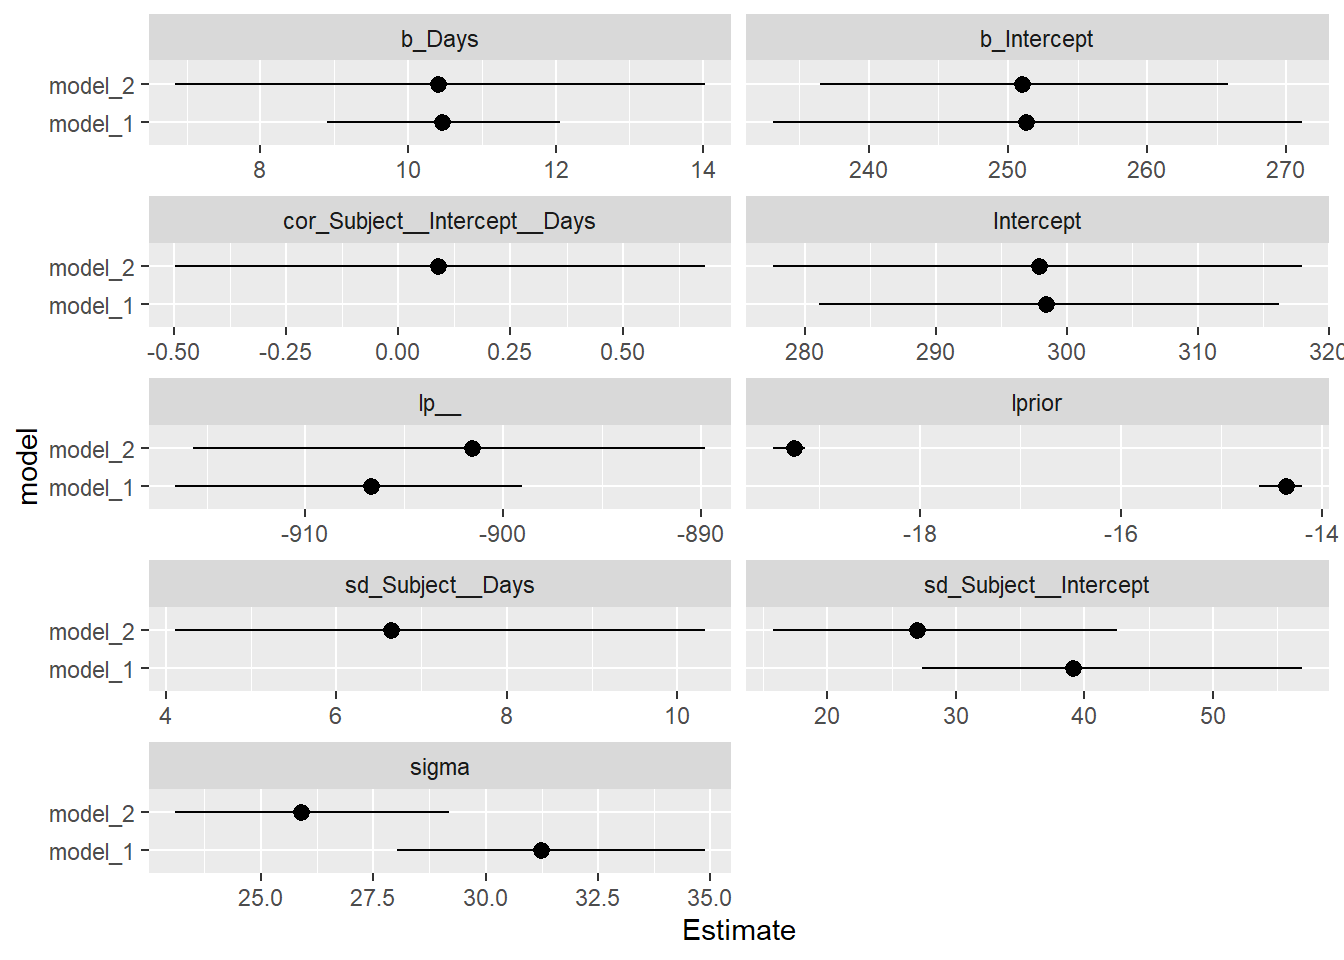
\includegraphics[width=0.8\textwidth,height=\textheight]{2021-04-12-models_files/figure-pdf/fig1-1.pdf}

\subsection{Model comparison}\label{model-comparison}

As part of the build pipeline, we computed a leave-one-out information
criteria (LOOIC) and LOO-weighted Bayesian R-squared statistic. Let's
look at the R2 first.

\begin{Shaded}
\begin{Highlighting}[]
\FunctionTok{loo\_R2}\NormalTok{(model\_1)}
\end{Highlighting}
\end{Shaded}

\begin{verbatim}
    Estimate Est.Error      Q2.5     Q97.5
R2 0.6604625 0.0480215 0.5561477 0.7439333
\end{verbatim}

\begin{Shaded}
\begin{Highlighting}[]
\FunctionTok{loo\_R2}\NormalTok{(model\_2)}
\end{Highlighting}
\end{Shaded}

\begin{verbatim}
    Estimate  Est.Error      Q2.5     Q97.5
R2 0.7447408 0.05599745 0.6170603 0.8363049
\end{verbatim}

This comparison would favor the second model.

Let's compare the LOOIC values. The second model has lower LOOIC values.

\begin{Shaded}
\begin{Highlighting}[]
\FunctionTok{loo}\NormalTok{(model\_1)}
\end{Highlighting}
\end{Shaded}

\begin{verbatim}

Computed from 4000 by 180 log-likelihood matrix.

         Estimate   SE
elpd_loo   -884.9 14.4
p_loo        19.3  3.4
looic      1769.8 28.8
------
MCSE of elpd_loo is 0.1.
MCSE and ESS estimates assume MCMC draws (r_eff in [0.5, 2.0]).

All Pareto k estimates are good (k < 0.7).
See help('pareto-k-diagnostic') for details.
\end{verbatim}

\begin{Shaded}
\begin{Highlighting}[]
\FunctionTok{loo}\NormalTok{(model\_2)}
\end{Highlighting}
\end{Shaded}

\begin{verbatim}

Computed from 4000 by 180 log-likelihood matrix.

         Estimate   SE
elpd_loo   -861.4 22.5
p_loo        34.4  8.7
looic      1722.8 45.1
------
MCSE of elpd_loo is NA.
MCSE and ESS estimates assume MCMC draws (r_eff in [0.5, 1.3]).

Pareto k diagnostic values:
                         Count Pct.    Min. ESS
(-Inf, 0.7]   (good)     176   97.8%   861     
   (0.7, 1]   (bad)        3    1.7%   <NA>    
   (1, Inf)   (very bad)   1    0.6%   <NA>    
See help('pareto-k-diagnostic') for details.
\end{verbatim}

We could report a difference.

\begin{Shaded}
\begin{Highlighting}[]
\FunctionTok{loo\_compare}\NormalTok{(model\_1, model\_2)}
\end{Highlighting}
\end{Shaded}

\begin{verbatim}
        elpd_diff se_diff
model_2   0.0       0.0  
model_1 -23.5      11.8  
\end{verbatim}

These would have to multiplied by -2 to be on the deviance scale.

\bookmarksetup{startatroot}

\chapter{Apr.~15, 2021 (Data
exploration)}\label{apr.-15-2021-data-exploration}

Source: 2021-04-11-data-exploration.rmarkdown

Let's read in our cached dataset.

\begin{Shaded}
\begin{Highlighting}[]
\FunctionTok{library}\NormalTok{(tidyverse)}
\end{Highlighting}
\end{Shaded}

\begin{verbatim}
-- Attaching core tidyverse packages ------------------------ tidyverse 2.0.0 --
v dplyr     1.1.4     v readr     2.1.5
v forcats   1.0.0     v stringr   1.5.1
v ggplot2   3.5.1     v tibble    3.2.1
v lubridate 1.9.4     v tidyr     1.3.1
v purrr     1.0.2     
-- Conflicts ------------------------------------------ tidyverse_conflicts() --
x dplyr::filter() masks stats::filter()
x dplyr::lag()    masks stats::lag()
i Use the conflicted package (<http://conflicted.r-lib.org/>) to force all conflicts to become errors
\end{verbatim}

\begin{Shaded}
\begin{Highlighting}[]
\NormalTok{data }\OtherTok{\textless{}{-}}\NormalTok{ targets}\SpecialCharTok{::}\FunctionTok{tar\_read}\NormalTok{(sleep\_data)}
\end{Highlighting}
\end{Shaded}

This is the \texttt{sleepstudy} dataset (\textbf{belenky2003?}) from the
lme4 package (\textbf{lme4-paper?}). It had repeated measurements of
reaction times nested in participants.

\begin{Shaded}
\begin{Highlighting}[]
\FunctionTok{head}\NormalTok{(data)}
\end{Highlighting}
\end{Shaded}

\begin{verbatim}
# A tibble: 6 x 3
  Reaction  Days Subject
     <dbl> <dbl>   <dbl>
1     250.     0     308
2     259.     1     308
3     251.     2     308
4     321.     3     308
5     357.     4     308
6     415.     5     308
\end{verbatim}

\begin{Shaded}
\begin{Highlighting}[]
\FunctionTok{count}\NormalTok{(data, Subject)}
\end{Highlighting}
\end{Shaded}

\begin{verbatim}
# A tibble: 18 x 2
   Subject     n
     <dbl> <int>
 1     308    10
 2     309    10
 3     310    10
 4     330    10
 5     331    10
 6     332    10
 7     333    10
 8     334    10
 9     335    10
10     337    10
11     349    10
12     350    10
13     351    10
14     352    10
15     369    10
16     370    10
17     371    10
18     372    10
\end{verbatim}

\begin{Shaded}
\begin{Highlighting}[]
\FunctionTok{count}\NormalTok{(data, Days)}
\end{Highlighting}
\end{Shaded}

\begin{verbatim}
# A tibble: 10 x 2
    Days     n
   <dbl> <int>
 1     0    18
 2     1    18
 3     2    18
 4     3    18
 5     4    18
 6     5    18
 7     6    18
 8     7    18
 9     8    18
10     9    18
\end{verbatim}

We can plot all the participants' data.

\begin{Shaded}
\begin{Highlighting}[]
\FunctionTok{ggplot}\NormalTok{(data) }\SpecialCharTok{+} 
  \FunctionTok{aes}\NormalTok{(}\AttributeTok{x =}\NormalTok{ Days, }\AttributeTok{y =}\NormalTok{ Reaction) }\SpecialCharTok{+} 
  \FunctionTok{geom\_line}\NormalTok{(}\FunctionTok{aes}\NormalTok{(}\AttributeTok{group =}\NormalTok{ Subject)) }\SpecialCharTok{+} 
  \FunctionTok{stat\_smooth}\NormalTok{(}\AttributeTok{se =} \ConstantTok{FALSE}\NormalTok{, }\AttributeTok{method =} \StringTok{"lm"}\NormalTok{, }\AttributeTok{size =} \DecValTok{2}\NormalTok{, }\AttributeTok{formula =}\NormalTok{ y }\SpecialCharTok{\textasciitilde{}}\NormalTok{ x)}
\end{Highlighting}
\end{Shaded}

\begin{verbatim}
Warning: Using `size` aesthetic for lines was deprecated in ggplot2 3.4.0.
i Please use `linewidth` instead.
\end{verbatim}

\begin{figure}[H]

{\centering 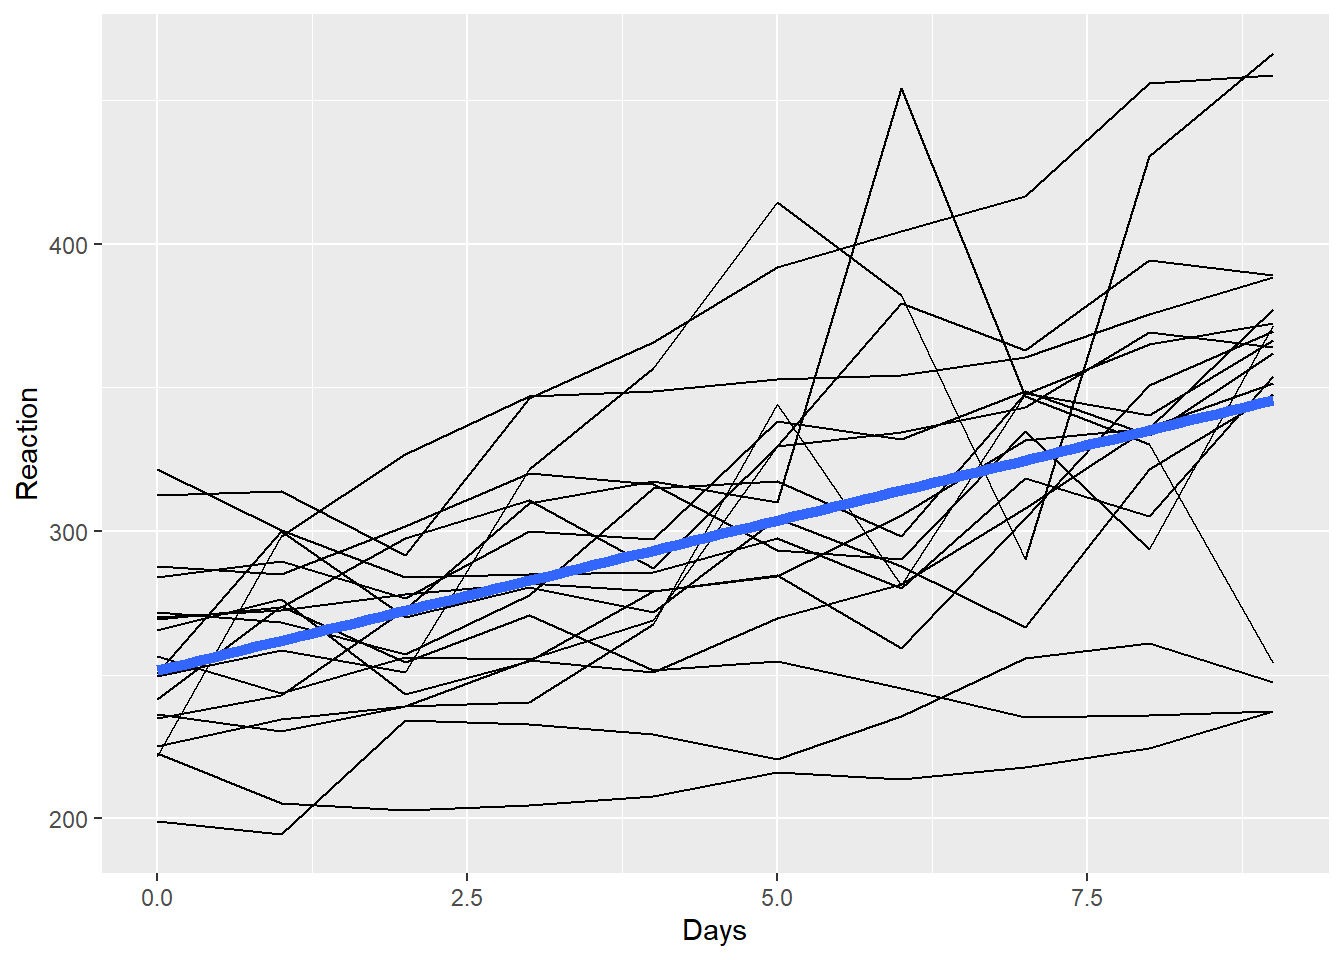
\includegraphics[width=0.8\textwidth,height=\textheight]{2021-04-11-data-exploration_files/figure-pdf/spaghetti-1.pdf}

}

\caption{Spaghetti plot of individual participant's data and group
mean.}

\end{figure}%



\end{document}
